% Journal:
%   Journal of Ambient Intelligence and Smart Environments (JAISE), IOS Press
%   Web Intelligence and Agent Systems: An International Journal (wias)
% Latex 2e
% Test file iosart2c.tex

%[seceqn,secfloat,secthm,crcready]

% options: wias, jaise
\documentclass{iosart2c}


\usepackage[T1]{fontenc}
\usepackage{times}%

%\usepackage{natbib}
\usepackage[numbers]{natbib}

\usepackage{hyperref}
\usepackage{amsmath}
\usepackage{dcolumn}
%\usepackage{endnotes}
\usepackage{graphics}


%========================== MY PACKAGES ================================%

%pseudocode
\usepackage{algorithm}
\usepackage{algpseudocode}

%draw artificial neural networks
\usepackage{neuralnetwork}
\usepackage{xpatch}
\makeatletter
\xpatchcmd{\linklayers}{\nn@lastnode}{\lastnode}{}{}
\xpatchcmd{\linklayers}{\nn@thisnode}{\thisnode}{}{}
\makeatother

%figures
\usepackage{graphicx}
\usepackage{graphics}
\usepackage{caption}
\usepackage{subcaption} %subimagenes

%math
\usepackage{amsmath,amssymb,amsfonts,amsthm} %for mathematics fonts 
\usepackage{stmaryrd}

%For ORCID logo
\usepackage{svg}



%========================== MY PACKAGES ================================%




\newcolumntype{d}[1]{D{.}{.}{#1}}


\firstpage{1} \lastpage{5} \volume{1} \pubyear{2009}


\begin{document}
\begin{frontmatter}                           % The preamble begins here.

%
%\pretitle{Pretitle}
\title{Evolving neural networks for threat process mitigation with autoencoder-based fitness functions.}

\runningtitle{Evolving neural networks for threat process detection using autoencoder to build a fitness function.}
%\subtitle{Subtitle}


\author[A,B]{\fnms{Henry D.} \snm{Navarro H.}\thanks{Corresponding author. Henry D. Navarro H., E-mail: contact@henrynavarro.org.}},
\author[B]{\fnms{Héctor} \snm{Bullejos}},
\author[B]{\fnms{Carmelo} \snm{Garrido}}
and
\author[B]{\fnms{Elena} \snm{Naranjo}}
\runningauthor{H. Navarro et al.}
\address[A]{Research and Development Lab, Vision Analytics, Avenida de Europa 19, 28224, Pozuelo de Alarcón, Madrid, Spain.\\
E-mail: contact@henrynavarro.org}
\address[B]{R\&D Department, Capgemini Engineering, Calle Campezo, 1, 28022, Madrid, Spain.\\
E-mail: engineering@capgemini.com}

\begin{abstract}
Threat detection and mitigation is a crucial aspect of cybersecurity research, and researchers have dedicated significant efforts to developing effective methods for identifying and responding to various types of threats, such as viruses and phishing attacks. Once an intruder has gained access to a system, it is essential to detect any malicious processes and prevent them from causing harm. In this paper, it is presented a real-time hybrid method for detecting and mitigating malicious processes on a simulated network system. This approach combines deep neural networks and evolutionary algorithms with an autoencoder-based fitness function and detects in real-time anomalous behavior in each device connected to the network.
\end{abstract}

\begin{keyword}
Neuroevolution \sep Genetic Algorithms \sep Threat detection \sep Autoencoders \sep Deep Neural Networks
\end{keyword}

\end{frontmatter}



\section{Introduction}
Deep neuroevolution, autoencoders, and cybersecurity are three interrelated areas that have the potential to significantly impact the field of information security. Deep neuroevolution refers to the use of evolutionary algorithms to optimize artificial neural networks, which can be used to improve the accuracy and efficiency of various machine learning tasks. Autoencoders, on the other hand, are a type of neural network that can be used to learn efficient representations of data, and have been applied to a wide range of problems including dimensionality reduction, anomaly detection, and data compression. In the context of cybersecurity, these techniques can be used to improve the ability of systems to detect and mitigate various cyber threats, such as malware, phishing attacks, and network intrusions.

To study the effects of malicious processes, a virtual network was created consisting of 20 virtual instances using open source software. It was assumed that the malicious process had already infiltrated the system using techniques such as ransomware or social engineering. System data was collected from these virtual instances using open source libraries and used to train neural networks and apply evolutionary algorithms based on deep neuroevolution to detect and terminate the malicious process. This controlled environment facilitated the study of the behavior of malicious processes and the development of effective methods for detecting and responding to them

Evolve neural networks has been used in different tasks but mainly in train neural networks to play video games \cite{deepGA, neuroevolution1, neuroevolution2}, although there are other applications as music generation \cite{neuroevolution3} and modelling biological phenomena \cite{neuroevolution4}. These neural network training methods rely on genetic algorithm operations to obtain the best agent to perform a specific task. However, there is not too much research related to this topic and cybersecurity as it is shown in the Section \ref{relatedwork}.

Evolutionary algorithms rely on a fitness function to identify the best agents in each generation. In this proposed method, the best agents are those that are able to ``kill'' the malicious process, returning the virtual instances to their ``normal states''. To determine the normal state of an instance, an autoencoder neural network is used. This neural network learns the healthy state of each instance and calculates the mean squared error (MSE) between its inputs and outputs. The closer the MSE is to zero, the healthier the state of the instance. The best agents are chosen according to this criterion and the malicious process is terminated using a simple command in any Linux based system (\texttt{kill}).


\section{Related work}\label{relatedwork}

Autoencoders are neural networks that consist of an encoder to generate a vector of features in the latent space (of smaller dimension) and from the input data and a decoder, which seeks to reconstruct the input data from this latent vector \cite{autoencoders_nlp1}. This type of neural networks are used in anomaly detection \cite{anomaly1, anomaly3, anomaly4}, natural language processing \cite{autoencoders_nlp1} and dimensionality reduction \cite{dimred1, dimred2}.

It has been demonstrated by other researchers that autoencoders can be used to detect other types of threats, such as Denial of Service attacks (\cite{autoencoderdos}). In their paper, an autoencoder is used to classify different types of Denial of Service attacks. The goal is not only to classify the state of a virtual machine as healthy or infected, but also to quantify the level of infection of a virtual instance. To achieve this, the autoencoder neural network is trained solely on healthy state data and the mean squared error (MSE) is used as a fitness function to select the best agents for threat detection. The lower the MSE, the healthier the state of the instance.

As for deep neuroevolution, there are no direct applications in the field of threat mitigation. However, other researchers have used genetic algorithms to improve network security \cite{GA1, GA2, GA3}. In most of these papers, binary genes are used to block or detect certain network attacks, such as Syn-Flood and Smurf. To do so, common operations in genetic algorithms such as selection, crossover, and mutation are applied.

There have been several investigations into malware detection using deep neural networks \cite{malwarednn1, malwarednn2,malwarednn3}. However, these researchers train their models using gradient-based algorithms. In this paper, an alternative method for training a neural network to detect malicious processes that create idle tasks that affect common system values such as CPU, memory RAM, and hard drive is presented. By detecting and terminating these processes, the healthy state of a virtual instance can be restored using a genetic algorithm with an autoencoder-based fitness function.

Therefore, the main contributions of this paper are:
\begin{enumerate}
	\item In \cite{autoencoderdos}, autoencoders are used as a classification neural network to detect and classify Denial of Service attacks. In the current paper, it is trained an autoencoder to detect anomalies caused by malicious processes that affect common parameters of the virtual instance. 
	\item Genetic algorithms have been used to improve security \cite{GA1, GA2, GA3}, but in the proposed method, it is used an autoencoder-based fitness function to evolve neural networks and select the best agents.
	\item In \cite{autoencoder3}, a comparison of different autoencoder architectures is conducted, while the proposed model in the current paper can detect any anomaly in each instance.
	\item Other hybrid methods have been proposed \cite{hybrid1, hybrid2}, but these methods are only used to detect system threats, while the proposed method generates agents that mitigate system threats and are trained using a non-gradient-based algorithm.
\end{enumerate}

\section{Methodology}

\subsection{Network simulation}

The virtual network to emulate the attacks was built and simulated based on the fact that an intruder had already obtained access to the network and already represents an internal threat, that is, the file that executes the malicious process is already found in the virtual instances. A network architecture with 20 instances has been virtualized using a network orchestrator with 4 physical machines.

These instances have their system data sent to a NoSQL database, where the variables explained in the Section \ref{dataset_autoencoder} are monitored and used to develop the proposed models.


\subsection{Dataset}\label{dataset_autoencoder}

To create the dataset, the normal traffic was first extracted from a virtualized environment to obtain ``healthy'' data for the system. A software tool was used to extract 97 features related mainly to CPU usage, memory RAM usage, and hard drive usage, which were divided into 10 main groups. Next, a cyber attack was introduced into each instance of the virtualized network and data was extracted to create an additional class: a malicious process called  ``Logic Bomb'', which was developed by the team. It affects the regular parameters such as CPU, memory, and disk by creating idle processes.

\subsubsection{Central Processing Unit (CPU) features}
They refer to the load characteristics that the CPU of the instance may have. A malicious process acting on the instances is expected to drive CPU usage across the entire instance in order to crash it.\\


\subsubsection{Core features}
These features are similar to CPU variables, with the difference that they are disaggregated by core. Due to how virtualized instances have been created (1GB of memory, 1 core only), these variables are expected to have a high correlation with the CPU variables.


\subsubsection{Disk Input/Output (Disk I/O) features}
Disk I / O operations include both read and write or Input / Output (usually defined in KB / s) involving a physical disk. In simple words, it is the speed with which the data transfer takes place between the hard disk drive and RAM, or basically it measures the input / output time of the active disk. It is a performance measure and is therefore used to characterize storage disks as HDD, SSD, and SAN. A malicious process is expected to constantly perform read and write operations to cause a saturation of this hardware.

\subsubsection{Entropy}
Entropy available on the system.

\subsubsection{Filesystem}

This set of features refer to file system statistics on disk. Some malicious processes create an infinite loop that creates files indefinitely in order to saturate it.

\subsubsection{Memory Swap}

When the physical memory or RAM in the system becomes full, the \textit{Memory Swap} is used. In this process, the inactive pages of the memory are moved to the swap space, creating more memory resources. This space is especially useful for systems that do not have RAM; however, it is slower to access because it is located on the hard drive and should not be considered as an alternative to RAM. As mentioned previously, a malicious process is expected to crash the RAM memory and then begin consuming the resources of the swap memory.


\subsubsection{Memory hugepages}

Hugepages are useful in managing virtual memory on Linux systems. As the name implies, they help manage large pages in memory that are larger than the default (usually 4KB). Hugepages is useful for both 32-bit and 64-bit configurations. Hugepages sizes can range from 2MB to 256MB, depending on the kernel version and hardware architecture. A malicious process is expected to increase the values of this variable.


\subsubsection{Socket summary}
These variables refer to the summary of open socket metrics in the system. A socket is nothing more than a communication channel between two programs that run on different computers or even on the same computer. Malicious processes seeking to attack the network are expected to affect these variables.

\section{Anomaly detection classification for fitness function}\label{autoencoder_section}

An autoencoder neural network is an unsupervised learning algorithm that applies backpropagation, configuring the target values to be equal to the inputs. That is, the response variable that the machine learning algorithm tries to learn is such that $y^{(i)} = x^{(i)} $, where $x^{(i)} = \{x^{(1)}, x^{(2)}, \ldots, x^{(n)} \} $ are the input variables detailed in Section \ref{dataset_autoencoder} and the Appendix \ref{appx_variables}.\\

\subsection{Autoencoder architecture}\label{autoencoder_architecture}

An autoencoder consists of two parts: an encoder, denoted as $f_{\phi}$, and a decoder, denoted as $g_{\theta}$. The entire autoencoder neural network can be represented as $h_{W, b} = g_\theta \circ f_\phi$, where $W$ and $b$ represent the weight matrix and bias vector of the neural network, and $h$ represents the final transformation function or hypothesis.

Next, $n_l$ denotes the number of layers in the network. In this case, a network with three hidden layers was taken, therefore $n_l=5$. The $l$-th layer is denoted as $L_l$, therefore $L_1$ is the input layer and $L_{n_l}$ denotes the output layer. The parameters $(W,b)=(W^{(i)},b^{(i)})$, with $i=1,\ldots,5$ are also denoted, where $W^{(l)}$ represents the weight matrices (weights) of each layer and $b^{(i)}$ represents the bias vector (bias) associated with the connections between unit (neuron) $j$ in layer $l$ and unit $i$ in layer $l+1$. Similarly, the activation function that ``connects'' layer $l-1$ with layer $l$ is denoted as $f_{\cdot l}$. Finally, $s_i$ denotes the number of neurons (units) in layer $i$.
 
To reduce the dimensionality of the dataset, a selection of variables is made, as explained in the results Subsection \ref{results_autoencoder}. The number of neurons in the encoder is selected such that $s_i=\left\llbracket\frac{s_{i-1}}{2}\right\rrbracket$ (half the number of neurons in the previous layer), while in the decoder, $s_i=\left\llbracket 2\times s_{i-1} \right\rrbracket$ (double the number of neurons in the previous layer). The symbol $\llbracket \cdot \rrbracket$ represents the integer part of a real number.

Like any neural network, it requires activation functions that allow connecting all the units (neurons) of each layer. For the autoencoder, the  activation functions are shown in Eqs. (\ref{activations_f})
\begin{eqnarray}
\begin{aligned} \label{activations_f}
f_{\cdot 2} &= \tanh(x)=\frac{e^{x}-e^{-x}}{ e^{x}+e^{-x}},  \\
f_{\cdot 3} &= ReLU(x) = x^+ = \max(0, x), \\
f_{\cdot 4} &= f_{\cdot 2} = \tanh(x)=\frac{e^{x}-e^{-x}}{ e^{x}+e^{-x}},  \\
f_{\cdot 5} &= f_{\cdot 3} = ReLU(x) = x^+ = \max(0, x)
\end{aligned}
\end{eqnarray}


$a_i^{(l)}$ denotes the activation (the value at the output) of the unit $i$ in the layer $l$. For $l=1$, the notation $a_i^{(1)}=x_i$ is used to denote the $i$-th input as shown in Eqs (\ref{z_ia_i}).
\begin{eqnarray}
\begin{aligned} \label{z_ia_i}
z^{(l)}&=W^{(l-1)}a^{(l-1)}+b^{(l-1)}\\
a^{(l)}&=f_{\cdot l}(z^{(l)})
\end{aligned}
\end{eqnarray}
Graphically, the architecture of the autoencoder can be seen in Figure \ref{fig:architecture_autoencoder}.


\begin{figure*}[h!]
\centering
\begin{neuralnetwork}[height=9.5,nodespacing=1cm,nodesize=20pt,  layerspacing=3.6cm][h]

    %comandos previos
    \newcommand{\x}[2]{\ifthenelse{\equal{#2}{0}}{$b_0$}{\ifnum #2=8 $x_n$ \else $x_#2$ \fi}} %si es el índice cero, entonces le asignas b0, sino si es la neurona 8, lo cambias por el índice n
    \newcommand{\ffirst}[2]{\ifthenelse{\equal{#2}{0}}{$b_1$}
    {\ifnum #2=4 $a_{\frac{n}{2}}^{(2)}$ \else $a_{#2}^{(2)}$ \fi}}
    \newcommand{\fsecond}[2]{\ifthenelse{\equal{#2}{0}}{$b_2$}
    {\ifnum #2=3 $a_{\frac{n}{4}}^{(3)}$ \else $a_{#2}^{(3)}$ \fi}}
    \newcommand{\fthird}[2]{\ifthenelse{\equal{#2}{0}}{$b_3$}
    {\ifnum #2=4 $a_{\frac{n}{2}}^{(4)}$ \else$a_{#2}^{(4)}$ \fi}}
    \newcommand{\xhat}[2]{\ifthenelse{\equal{#2}{0}}{$b_0$}{\ifnum #2=8 $\hat{x}_n$ \else $\hat{x}_#2$ \fi}}
    
    %red neuronal
    \hspace{-0.75cm}
    \inputlayer[count=8, bias=true,exclude={7},title=Input\\layer, text=\x]
    \hiddenlayer[count=4, bias=true,exclude={3},title={$L_2$\\$f_{\cdot 2} = \tanh(x)$}, text=\ffirst] 
    \linklayers[not from={7},not to={3}] %para que no dibuje la flecha desde la neurona 7
    \hiddenlayer[count=3, bias=true,exclude={2}, title={$L_3$\\$f_{\cdot 3} = ReLU(x) $}, text=\fsecond]
    \linklayers[not from={3},not to={2}]
    \hiddenlayer[count=4, bias=true,exclude={3}, title={$L_4$\\$f_{\cdot 4} = \tanh(x)$}, text=\fthird]
    \linklayers[not from={2},not to={3}]
    \outputlayer[count=8, exclude={7},title={Output layer\\$\hat{x}_i=a_{i}^{(5)}$}, text=\xhat]
    \linklayers[not to={7},not from={3}]
    
    
     % draw dots
    \path (L0-6) -- node{$\vdots$} (L0-8);
    \path (L1-2) -- node{$\vdots$} (L1-4);
    \path (L2-1) -- node{$\vdots$} (L2-3);
    \path (L3-2) -- node{$\vdots$} (L3-4);
    \path (L4-6) -- node{$\vdots$} (L4-8);
    
\end{neuralnetwork}
\caption{Architecture of the neural network of the autoencoder type used for anomaly detection}
\label{fig:architecture_autoencoder}
\end{figure*}


The autoencoder is trained using the well-known stochastic gradient descent algorithm with 60 epochs. The next step is to determine the decision threshold that will be used to classify instances as infected. That is, any instance with a value greater than this threshold will be considered infected or exhibiting anomalous behavior. To determine this threshold, the mean squared error between the input data and the output of the trained autoencoder is used, as shown in Algorithm \ref{autoencoder_anomalias}.


\begin{algorithm}[h!]
\caption{Anomaly detection algorithm with the autoencoder}\label{autoencoder_anomalias}
\textbf{Input:} Validation dataset $X_{val}=\{x^{(1)},\ldots,x^{(n)}\}$, autoencoder $h_{W,b}=g_\theta \circ f_\phi$.\\ Train dataset with normal behaviour  $X$, Anomaly train data $x^{(i)}$ $i = 1,...,N$, threshold $\alpha$\\
\begin{algorithmic}[1]
\State $\phi$, $\theta$ $\xleftarrow{}$ Train the autoencoder with normal data $X$
\For{i=1 to N}
    \State $MSE(i) = \lVert x^{(i)} - g_\theta(f_\phi(x^{(i)})\rVert_2^2$ \Comment{Mean Square Error (MSE)}
    \If{$MSE(i) > \alpha$}
        \State$x^{(i)}$ is an anomaly
        \State pred$\xleftarrow{}$1
    \Else 
        \State$x^{(i)}$ is not an anomaly
        \State pred$\xleftarrow{}$0
    \EndIf
\EndFor
\end{algorithmic}
\textbf{Output:} Vector of classifications.\\
\end{algorithm}


Additionally, to meet the objective, it is necessary to determine the threshold at which an anomaly can be identified. To find this decision threshold, the mean squared errors for the training data (healthy instances) will be tested and the optimal one that maximizes accuracy in the confusion matrix will be determined, as shown in Algorithm \ref{obtener_umbral}.


\begin{algorithm}
\caption{Obtaining the optimal $\alpha$ threshold for anomaly detection}\label{obtener_umbral}
\textbf{Input:} Train dataset $X_{train}=\{X_{train}^{(1)},\ldots,X_{train}^{(n)}\}$, Validation dataset $X_{val}=\{X_{val}^{(1)},\ldots,X_{val}^{(n)}\}$, autoencoder $h_{W,b}$.\\

\begin{algorithmic}
\State $\hat{X}_{train} \xleftarrow{} h_{W,b}(X_{train})$ \Comment{Evaluate the training data in the autoencoder.}
\State $Max\_MSE\_{train}\xleftarrow{}\max\left(\sum_{i=1}^n\left(X_{train}^{(i)}-\hat{X}_{train}^{(i)}\right)^2\right)$ \Comment{From the list above, the largest values of root mean square error are taken}
\State $\hat{X}_{val} \xleftarrow{} h_{W,b}(X_{val})$ \Comment{Same for validation data.}
\State $MSE_{val}\xleftarrow{}\sum_{i=1}^n\left(X_{val}^{(i)}-\hat{X}_{val}^{(i)}\right)^2$ 
\State $partition\xleftarrow{} Max\_MSE\_{train}/1000$
\State Initialize $\alpha$, $Accuracy_{optimal}$, $MSE_{optimal}$ with zero values.\\



\For{i=1 to 1000} \Comment{1000 threshold partitions are tested, from 0 to $Max\_MSE\_{train}$ and the best is saved:}
    \State $y_{val}^{(i)}\xleftarrow{}anomaly(MSE_{val},\alpha)$\Comment{Apply the Algoritmh \ref{autoencoder_anomalias} (vector of 1's y 0's)}
    \State $Accuracy_{current}\xleftarrow{}$ Get the accuracy from $(y_{val},y_{val}^{(i)})$
        \If{$Accuracy_{current}>Accuracy_{optimal}$} 
            \State $Accuracy_{optimal}\xleftarrow{}Accuracy_{current}$
            \State $\alpha\xleftarrow{}MSE_{current}$
        \EndIf
    \State $MSE_{current}\xleftarrow{}MSE_{current}+partition$
\EndFor\\
\end{algorithmic}
\textbf{Output:} Optimal threshold $\alpha$.\\
\end{algorithm}


\newpage



\section{Evolutionary algorithm approach}

\subsection{Features for agents}\label{variables}

To identify malicious processes in an instance, we will study certain features that may be indicative of such processes. These variables do not directly describe the instance itself, but rather the processes running on it, since there is no dataset of processes that have been classified as malicious. The hybrid machine learning and genetic algorithms must be able to detect and mitigate these processes, using the correct order (\texttt{kill} process or not). In this case, the variables have been grouped into four main categories.


\subsubsection{File descriptors}

The file descriptor is a non-negative integer that uniquely identifies the files opened in a session. Each process is allowed to have up to nine file descriptors open at one time. The bash shell reserves the first three file descriptors (0, 1, and 2) for special purposes \cite{shell_scripting2}. 

\subsubsection{Central Processing Unit (CPU)}

They refer to the load characteristics that the CPU may have for each process. A malicious process acting on the instances is expected to drive up CPU usage in order to crash it.\\

\subsubsection{Memory}

This set of variables refer to the RAM memory consumption that each process performs. A malicious process should carry out a high consumption of these type of resources. 


\subsubsection{Temporal features}

As the name indicates, in this set are the variables that are related to time.\\

\subsection{Architecture of the agents (neural networks) of the population} \label{arquitectura_agents}

Following the notation in the Section \ref{autoencoder_architecture}, the neural network has parameters $(W,b)=(W^{(1)},b^{(1)},W^{(2)},b^{(2)})$. That is, $W^{(1)} \in \mathbb {R}^{15x8}$, while $ W^{(2)} \in \mathbb {R}^{1x15}$. A softmax function is used as a network hypothesis. Thus, the hypothesis will be $h: \mathbb {R}^ {2} \rightarrow [0,1]^2 $ as the softmax function of the last layer of each neural network: 
\begin{equation}\label{softmax}
h_{W,b}(x)=\left(\frac{e^{a_1^{(3)}}}{\sum_{j=1}^2 e^{a_j^{(3)}}},\frac{e^{a_2^{(3)}}}{\sum_{j=1}^2 e^{a_j^{(3)}}}\right)
\end{equation}


Therefore, for the logical bomb attack, $n^{[2]}=2$. That is, a vector as it is shown in Eq. (\ref{P_kill}):


\begin{eqnarray}
\begin{aligned}\label{P_kill}
    (P_{\texttt{no}},P_{\texttt{kill}})=(&P(\texttt{no kill process } | \\
									    & X=x_1,\ldots,x_n),\\
                                         &P(\texttt{kill process } | \\
                                         & X=x_1,\ldots,x_n))
\end{aligned}
\end{eqnarray}

such that  $P_{\texttt{no}}+P_{\texttt{kill}}=1$, where $x_i$ are the monitored variables for that process, defined in Section \ref{variables}. So the activation function in the last hidden layer will be given by the function softmax in Eq. (\ref{softmax}).

The chosen neural network for this study can be seen in Figure \ref{fig:architecture_autoencoder}.

\begin{figure*}[h!]
\centering
\begin{neuralnetwork}[height=8,nodespacing=1cm,nodesize=20pt,  layerspacing=3.6cm][h]

    %comandos previos
    \newcommand{\x}[2]{\ifthenelse{\equal{#2}{0}}{$b_0$}
    {\ifnum #2=4 $x_n$ \else $x_#2$ \fi}} %si el índice=cero, asigna b0, sino si es la neurona 8, lo cambias por el índice n
    \newcommand{\ffirst}[2]{\ifthenelse{\equal{#2}{0}}{$b_1$}
    {\ifnum #2=6 $a_{15}$ \else $a_{#2}^{(2)}$ \fi}}
    \newcommand{\y}[2]{$y_#2$}
    
    %red neuronal
    \inputlayer[count=4, bias=true,exclude={3},title=Input\\layer, text=\x]
    \hiddenlayer[count=6, bias=true,exclude={5},title={$L_2$\\$f_{\cdot 2} = reLU(x)$}, text=\ffirst]
    \linklayers[not from={3},not to={5}] %para que no dibuje la flecha desde la neurona 7
    \outputlayer[count=2, title={Output layer\\$softmax(x)$}, text=\y]
    \linklayers[not from={5}]
    
    
     % draw dots
    \path (L0-2) -- node{$\vdots$} (L0-4);
    \path (L1-4) -- node{$\vdots$} (L1-6);

\end{neuralnetwork}
\caption{Neural network architecture used for attack mitigation.}
\label{arq_agent}
\end{figure*}


\subsection{Evolving Neural Networks}

Therefore, each agent is a neural network known as a multilayer perceptron (MLP) with $n^{[0]}=8$ \textit{input units} (neurons in the input layer), due to the variables of the processes to analyze (See Section \ref{variables}), $n^{[1]}=15$ \textit{hidden units} (neurons in the hidden layer) This design intention is to have twice as many neurons in the hidden layer as in the input layer, with $n^{[2]}=2$ \textit{output units} (neurons in the output layer). An illustration about the architecture of these agents is shown in Figure \ref{arq_agent}.

\subsection{Initialization}\label{sec_init}

There will be $\lambda$ neural networks (initial population size) per generation, where $\lambda$ is the maximum number of instances that can be virtualized in the environment according to computer resources. The weights $W_{ij}^{[l]}$ of the $\lambda$ neural networks are initialized using the general rule for establishing weights in a neural network, which is to set them close to zero without being too small. This is done using the \textsc{HeWeights} defined in Algorithm \ref{Hefunction}.


\begin{algorithm}[h!]
\caption{He Initialization}\label{Hefunction}
\begin{algorithmic}[1]
\Function{HeWeights}{agent}
\State n $\gets$ number of nodes of layer $l$  \Comment{agent is the neural network}
\State y $\gets$ $\frac{1.0}{\sqrt{n}}$
\State agent.weights $\gets$ $U(-y,y)$ \Comment{random numbers with distribution $U(-y,y)$}
\State return agent 
\EndFunction
\end{algorithmic}
\end{algorithm}

Therefore, the initialization operation of the deep neuroevolution algorithm is a configuration of $\lambda$ multilayer perceptrons with weights initialization $W_{ij}^{[l]}$ with uniform distribution as seen in the Algorithm \ref{init}.


\begin{algorithm}[h!]
\caption{Initialization}\label{init}
\hspace*{\algorithmicindent} \textbf{Input:} population size or number of agents $\lambda$, number of neurons in input each layer: $n^{[0]}, n^{[1]}, n^{[2]}$, weights initialization function $\phi$.
\begin{algorithmic}[1]
\State agents $\gets$ \text{empty list}
\For{$i = 1,\ldots,\lambda$}
\State init\_agent $\gets$ create a MLP with $n^{[0]}, n^{[1]}, n^{[2]}$ neurons in each layer and ReLU as activation function.
\State init\_agent $\gets$ \textsc{HeWeights}(init\_agent) \Comment{function that returns weights using He's initialization.}
\State agents[i] $\gets$ init\_agent \Comment{add to list the agent initialized}
\EndFor
\end{algorithmic}
\hspace*{\algorithmicindent} \textbf{Output:} $\lambda$ neural networks with He's initialization.
\end{algorithm}




\subsubsection{Evaluation}\label{evaluacion}

This operation determines the quality of the agents that result from the initialization or after each operation (selection, crossing, mutation, elitism). To do this, we use the pretrained autoencoder with healthy data. The autoencoder provides a measure through mean square error, as described in Section \ref{autoencoder_section}. This allows to assess the fitness of the agents.

The goal of this model is to provide a measure that allows for the detection of anomalies in the data of virtual instances. To do this, the evaluation operation is based on the mean square error (MSE) between the input data ${x_1,x_2,x_3,\ldots}$ (instance data) and the output data ${\hat{x}_1,\hat{x}_2,\hat{x}_3,\ldots}$ of the autoencoder.

Thus, the evaluation operator or \textit{fitness function} of the Deep Neuroevolution algorithm will be given by Eq. (\ref{fitness}):
\begin{equation}\label{fitness}
    fitness=MSE=\frac{1}{n^{[0]}}\sum_{i=1}^{n^{[0]}} (x_i-\hat{x}_i)^2
\end{equation}
where ${x_1,x_2,x_3,\ldots}$ are the input data of the autoencoder (instance data) and ${\hat{x}_1,\hat{x}_2,\hat{x}_3,\ldots}$ is the data in output the output of the autoencoder. \textbf{The closer the fitness function is to zero, the better the agent will be.} \\



\subsubsection{Selection and Crossing}

After the evaluation, those individuals/agents (from the $n$ neural networks) with the best fitness (Eq. (\ref{fitness})) should be selected, in the case of study, a fitness value closer to zero will be an indicator of better agent. \\

Now, within the operations that will defined are two of the most important: Selection and Crossing. For the first operation, the name is quite intuitive and it seeks to select the best agents according to the fitness function (the closer to zero, the better). The best $n_{top}$ will be selected, where
\begin{equation}\label{n_top}
    n_{top}=\left\llbracket\frac{-1+\sqrt{1+4\cdot2\cdot \lambda}}{2}\right\rrbracket+1
\end{equation}

and $\llbracket x\rrbracket$ is the \textit{floor} function. This is because the crossover operation requires reproducing $\lambda-1$ agents from the best ones, which requires a number $n_{top}$ such that $\sum_{i=1}^{n_{top}} i=\lambda$. Therefore, Eq. (\ref{n_top}) is the solution to the Eq. (\ref{eq_solve})
\begin{equation}\label{eq_solve}
	\frac{n_{top}(n_{top}+1)}{2}=\lambda,
\end{equation}
where $\lambda$ is the number of agents in the initial population $P_0$

The best $n_{top}$ agents are used to define the crossover operation, which aims to create a population of size $\lambda-1$ by combining the weights $W_{ij}$ of a ``father'' agent with those of several ``mother'' agents with a probability of $0.5$. This is a Bernoulli event, in which a coin is flipped and, if the result is heads, the offspring will inherit the weight $W_{ij}$ of the father; if the result is tails, it will inherit the weight $W_{ij}$ of the mother. The detailed algorithm can be seen in Algorithm \ref{selec_cross}.


\begin{algorithm}
\caption{Selection and Crossing}\label{selec_cross}
\begin{algorithmic}[1]
\State $n_{top}=\left\llbracket\frac{-1+\sqrt{1+4\cdot2\cdot\lambda}}{2}\right\rrbracket+1$
\Function{Selection and crossover}{agents,$n_{top}$}
\State agents\_top= select best $n_{top}$ agents from the list agents.
\State children= empty list
\State max\_id = 1 \Comment{Initialize a loop end parameter}
\While {\texttt{max\_id<=n-1}}
\For{\texttt{i = 1,\ldots,max\_id}}
\State mother=agents\_top[i] \Comment{Neural network mother}
\State father=agents\_top[max\_id] \Comment{Neural Network father}
\For{each unit of neural network $W_{ij}^{[parent]}$}
\State coin=$U(0,1)$ \Comment{Get random number with uniform distribution}
\State \textbf{If} coin$\leq0.5$ \textbf{then}
\State \hspace{0.5cm} $W_{ij}^{[children]}$=$W_{ij}^{[father]}$ \Comment{Update each weight of each unit}
\State \textbf{Else}
\State \hspace{0.5cm} $W_{ij}^{[children]}$=$W_{ij}^{[mother]}$ \Comment{Update each weight of each unit}
\EndFor
children[i]=new\_children
\EndFor
\EndWhile
\State \textbf{Return} children
\EndFunction
\end{algorithmic}
\end{algorithm}



\subsubsection{Mutation}

In evolutionary algorithms it is convenient that for the new descendants formed by selection and crossing, some of their genes (in this case the weights of the neurons) can be subjected to a mutation with a low random probability of a change. This implies that some weights of the neurons of the initial $\lambda$ neural networks, will be modified with a ``small'' change that depends on a value known as \textit{mutation power} \cite{deepGA}. This hyperparameter is called $\sigma$. 

The mutation occurs to maintain diversity within the population, without this operation, the values of the weights $W_{ij}$ of the neural networks (agents) would only maintain the values obtained from initialization.

The operation of adding a value $\sigma\cdot \mathcal{N}(0,1)$ with $\sigma=0.02$ to the weights $W_{ij}$ of the units (neurons) of each neural network is performed in order to allow these weights to vary beyond the values they have taken in the initialization operation (Algorithm \ref{init}). This value $\sigma$, which is very small and has a distribution of $\mathcal{N}(0,0.02^2)=\mathcal{N}(0,0.0004)$, prevents the weights from having extreme changes while allowing them to vary. This value can be considered analogous to the learning rate in the case of stochastic gradient descent and is defined in Algorithm \ref{mutation}.



\begin{algorithm}[h!]
\caption{Mutation} \label{mutation}
\begin{algorithmic}[1]
\State $\sigma=0.02$ \Comment{mutation power}
\State mutated\_children= empty list
    \Function{mutation}{children} \Comment{As input it needs the list returned by selection and crossover operation (Algorithm \ref{selec_cross})}
        \For{i = 1,\ldots,total of children}
            \For{each weight $W_{ij}$ of unit of neural network}
                \State $r_{norm}$= get random number $\mathcal{N}(0,1)$
                \State $W_{ij}$=$W_{ij}+\sigma\cdot r_{norm}$ \Comment{Update each weight of each unit}
                \State new\_children=assign to this neural network the weights $W_{ij}$.
            
\EndFor \\
        \State mutated\_children[i]=new\_children
\EndFor
\State \textbf{Return} mutated\_children
\EndFunction
\end{algorithmic}
\end{algorithm}



\subsubsection{Elitism}

The best agent mitigating the attack is selected as just one neural network, referred to as elitism. From the top $n_{top}$ (Eq. (\ref{n_top})) agents are selected, a process known as \textit{tournament elitism} is performed. This involves testing each agent (neural network) a total of $m$ times in the virtualized environment with the infected instances, and calculating the average \textit{fitness} (Eq. (\ref{fitness})) of these $m$ tests. This average determines which agent is the best after the $m$ executions. Finally, the elite agent (neural network) is added to the list of child agents (mutated\_children), preserving the best of all \textbf{unmutated} agents without any alteration, allowing the agent with the best attack mitigation characteristics to be kept. The Algorithm \ref{elitismo} explains how this operation is defined.


\begin{algorithm}[h!]
\caption{Elitism}\label{elitismo}
\begin{algorithmic}[1]
\State $n_{top}=\left\llbracket\frac{-1+\sqrt{1+4\cdot2\cdot \lambda}}{2}\right\rrbracket+1$
\Function{Elitism}{mutated\_children,agents,$n_{top}$}
\State agents\_top= select best $n_{top}$ agents from the list agents.
\For{i = 1,..., $n_{top}$}
    \State agent\_test = agents[i]
    \State fitness\_agent= empty list
    \State j=1
    \Repeat
        \State test the agent in the virtualized environment
        \State fitness\_agent[j]=calculate the fitness using Eq. (\ref{fitness}).
        \State j=j+1
    \Until{j=$m$}
\EndFor
\State fitness\_mean[i]=$\frac{1}{m}\sum^m_{j=1}$fitness\_agent[j]
\State elite=select agent with best fitness\_mean
\State new\_generation=add elite to mutated\_children
\State \textbf{Return} new\_generation
\EndFunction
\end{algorithmic}
\end{algorithm}


On the other hand, agents that kill all processes are penalized, as the neural network will learn to reduce the MSE given by the autoencoder based on killing all processes of the instance. When the agent tries to apply the \texttt{kill} command to all processes, the command is changed to not kill any processes. The neuroevolution algorithm is illustrated in Figure \ref{fig:diagneuroevolution}.

\begin{figure}[h!]
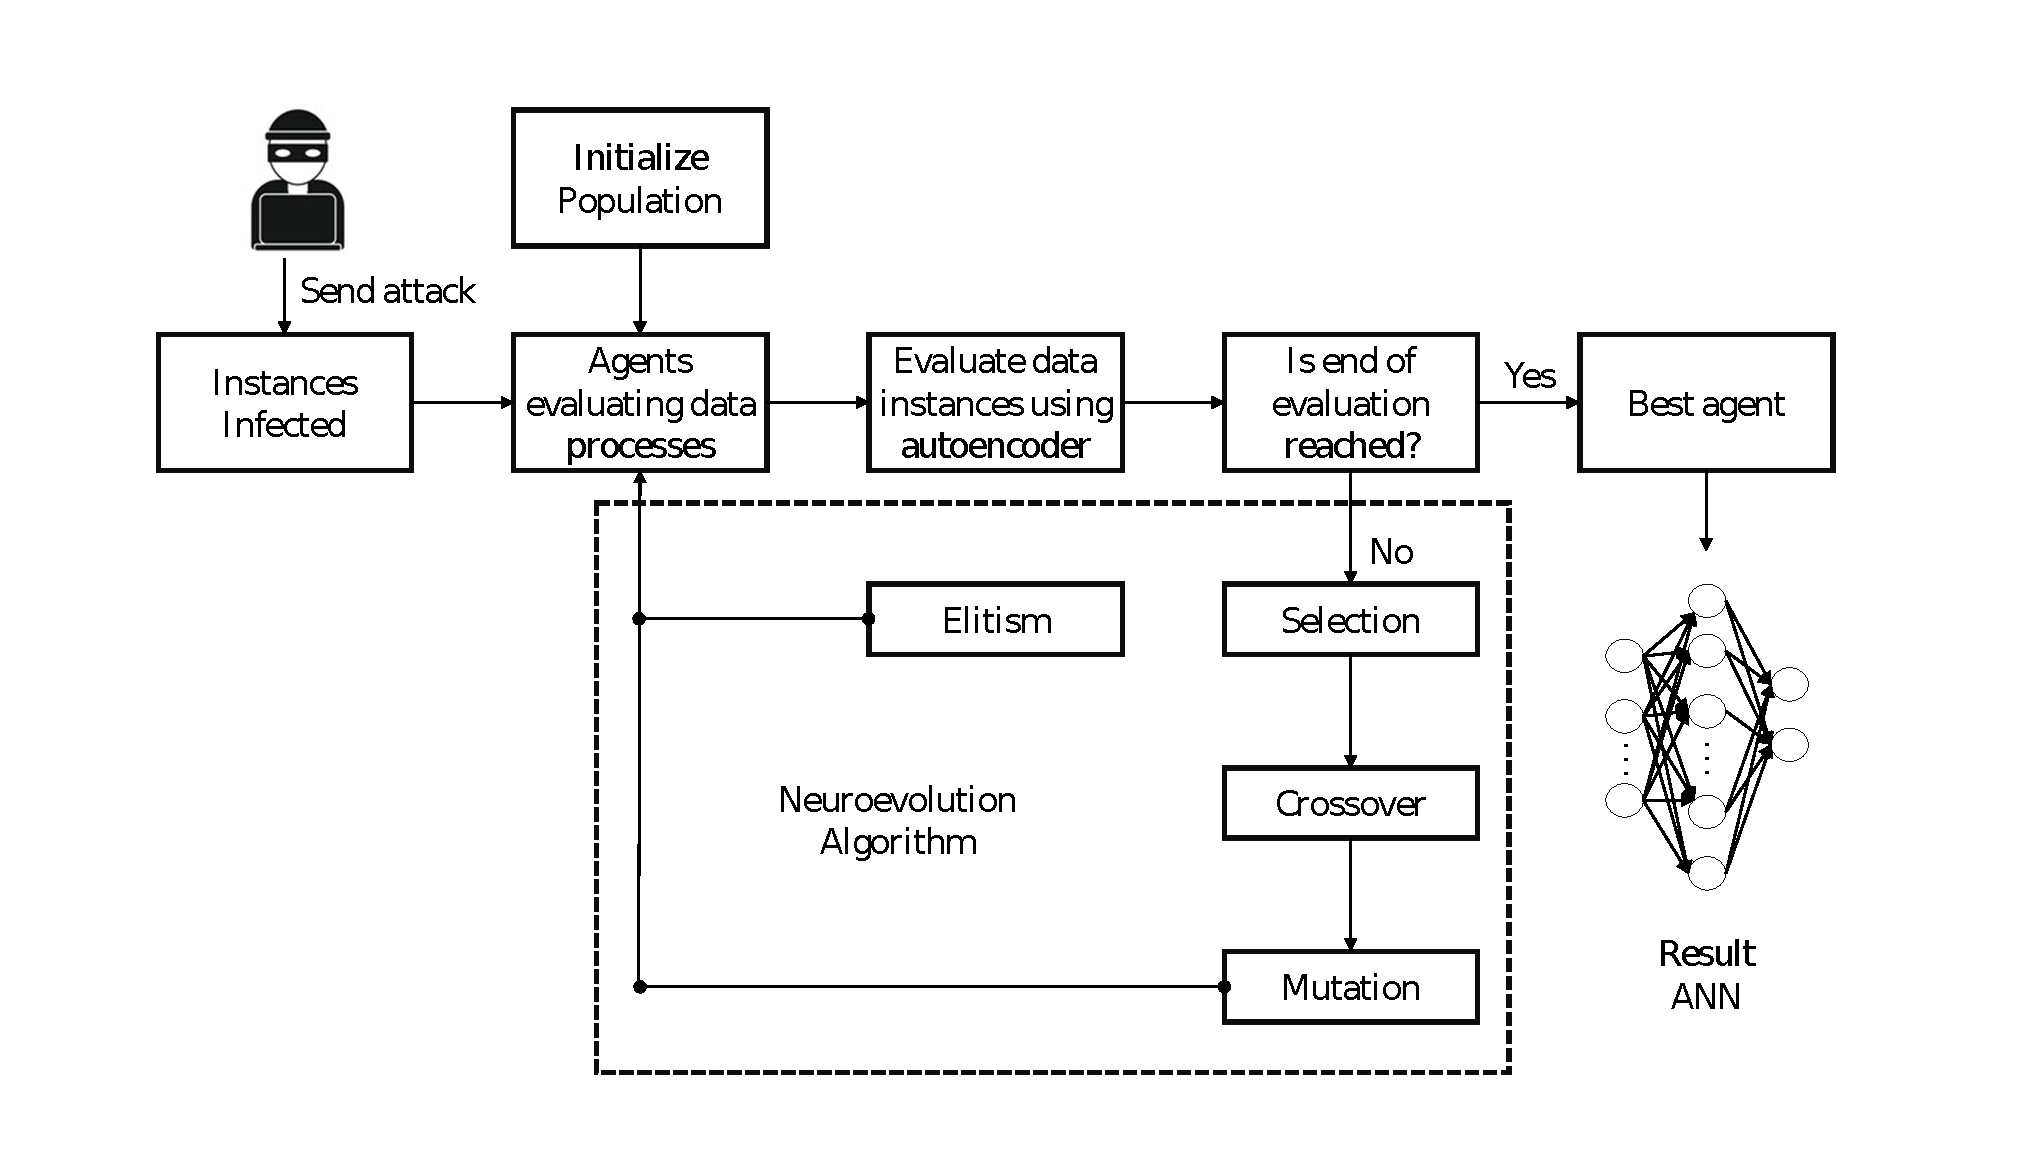
\includegraphics[width=0.51\textwidth]{figs/neuroevolution/diag_neuroevolution.eps}
\vspace{-0.5cm}
\caption{Neuroevolution algorithm flow.}
\label{fig:diagneuroevolution}
\end{figure}




\section{Experiments and Results}


\subsection{Feature selection}

Due to the high dimensionality of the data used to train the autoencoder, it is necessary to discard certain features in order to improve the performance of the model. To reduce the number of variables, a preliminary study of each variable was conducted, comparing the results between the different states of each instance. The first variables to be deleted were those that remained unchanged throughout the data extraction, regardless of the state of the virtual instance. Through this process, 26 of the 97 initial variables were eliminated. A short list of some of these variables can be seen in Table \ref{tab_cor}.

It is well known that multicollinearity in data can significantly reduce the predictive power of many machine learning models. While an autoencoder is not a linear model, it is still beneficial to reduce the high dimensionality of the data. One effective way to do this is by considering the correlation between variables.



\begin{table*}[h!]
\centering
\begin{tabular}{ccc}
\hline
Variable 1 & Variable 2 & Correlation \\ \hline
load 15 & load norm 15 & 1.0\\ 
memory used bytes & memory free & 1.0\\ 
filesystem free & filesystem available & 0.99\\ 
entropy available bits & entropy pct & 0.99\\ 
core idle pct & cpu idle pct & 0.99\\ 
cpu iowait pct & core iowait pct & 0.99\\ 
diskio io time & diskio write count & 0.99\\ 
process summary sleeping & process summary total & 0.98\\ 
cpu total pct & core idle pct & 0.98\\ 
fsstat total size used & fsstat total size free & 0.987\\ 
diskio iostat await & diskio iostat write await & 0.92\\ 
socket summary all count & socket summary udp all count & 0.91\\ 
diskio iostat queue avg size & diskio iostat busy & 0.90\\ \hline
\end{tabular}
\caption{Pearson correlation ($\rho$). List of some variables with correlation coefficient $\rho>0.90$.}
\label{tab_cor}
\end{table*}

To reduce multicollinearity in the data, we first identified variables that had a strong correlation with each other (a Pearson's correlation coefficient higher than 0.7). After examining the relationships between these variables, we conducted a study on the variables themselves to determine which ones were redundant. In order to have a more comprehensive understanding of the system, we also tried to retain at least one representative variable for each module. Through this process, 58 out of the 97 total variables were discarded."


\subsection{Results}


The results show that it is possible to determine the state of a instance using autoencoders and also detect malicious processes that affect the normal behaviour of a computer. So the results are presented in two steps: anomaly detection results and evolutionary algorithms for neural networks.


\subsubsection{Autoencoder model results}\label{results_autoencoder}

The autoencoder model was trained with only the healthy state of the data using the stochastic gradient descent algorithm with 60 epochs. The mean square error was monitored during the training process, the results are shown in Figure \ref{fig:autoencoder_variable_selected}.\\



\begin{figure}[h!]
\centering
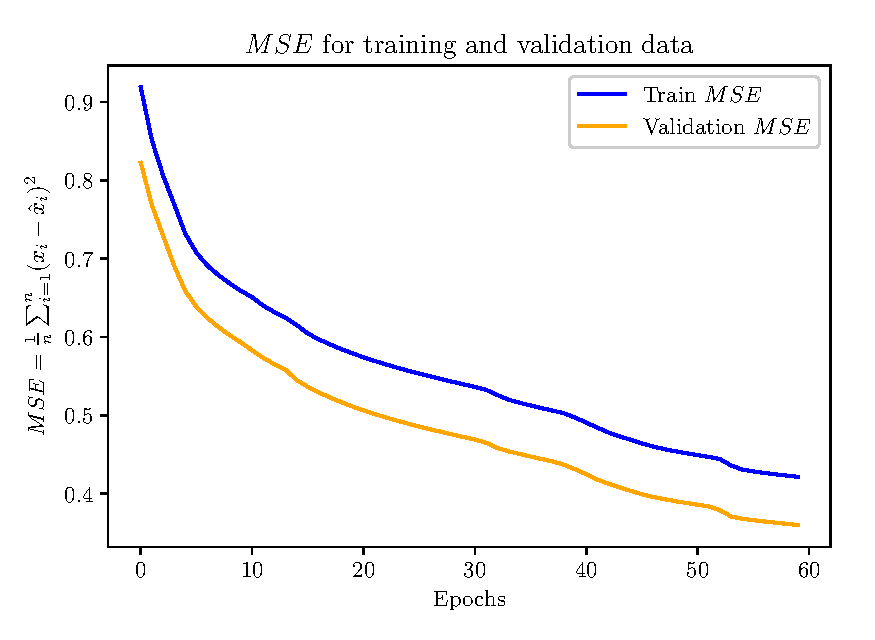
\includegraphics[scale=0.56]{figs/autoencoder/final_autoencoder.eps}
\caption{Epochs vs. $MSE$. Mean square error for a trained (Train) and validated (Validation) data for the autoencoder neural network with data from healthy machines after feature selection.}
\label{fig:autoencoder_variable_selected}
\end{figure}

After the model is trained, it is necessary to determine the decision threshold from which the state of the machine is considered an anomaly, for this, the Algorithm \ref{obtener_umbral} was used. Which gave as a result an optimal threshold $\alpha\approx 1.1945\ldots$, the closer value to this the state of the instance is, the greater the consideration will be as a healthy state of the instance. Therefore, the best ``parents'' will be those that after killing the processes, lead to the state of the instances at values closer to this $\alpha$. After the data extraction of anomaly values, the results of this analysis can be seen in Figure \ref{fig:reconstuction_LB}.\\

After the model is trained, it is necessary to determine the decision threshold at which the state of the machine is considered anomalous. To do this, we used Algorithm \ref{obtener_umbral}, which resulted in an optimal threshold $\alpha\approx 1.1945\ldots$. The closer the value of the state of the instance is to this threshold, the greater the consideration of it as a healthy state of the instance. Therefore, the best ``parents'' will be those that, after killing the processes, lead to the state of the instances with values that are below this $\alpha$. The results of this analysis can be seen in Figure \ref{fig:reconstuction_LB}.


\begin{figure}[h!]
\centering
\includegraphics[scale=0.56]{figs/autoencoder/reconstruccion_error_LB.eps}
\caption{Threshold decision from the mean square error (MSE). The red line represents the threshold decision $\alpha\approx1.1945\ldots$ to classify the anomaly.}
\label{fig:reconstuction_LB}
\end{figure}

With this decision threshold, a confusion matrix is obtained in order to consider the autoencoder not only as a anomaly detector but also as a classifier and to provide results about classification metrics. The results are shown in Table \ref{confusion_matrix}.


\begin{table}[h!]
\centering
\begin{tabular}{llll}
                                                &                                 & \multicolumn{2}{c}{Real}                                       \\ \cline{3-4} 
                                                & \multicolumn{1}{l|}{}           & \multicolumn{1}{l|}{L. Bomb} & \multicolumn{1}{l|}{Healthy} \\ \cline{2-4} 
\multicolumn{1}{c|}{Predicted} & \multicolumn{1}{l|}{L. Bomb} & \multicolumn{1}{l|}{1629}       & \multicolumn{1}{l|}{174}     \\ \cline{2-4} 
\multicolumn{1}{c|}{}                           & \multicolumn{1}{l|}{Healthy}    & \multicolumn{1}{l|}{135}        & \multicolumn{1}{l|}{5457}    \\ \cline{2-4} 
\vspace{0.001cm}
\end{tabular}
\caption{Classification considering  $MSE>\alpha$ is infected.}
\label{confusion_matrix}
\end{table}

A 10-fold cross validation is performed, and the performance measures (mean of the 10-fold results) shown in Eqs. (\ref{perf_measures}) are obtained.
\begin{eqnarray}\label{perf_measures}
\begin{aligned}
\hspace{-0.3cm} Accuracy  &= \hspace{0.5cm} \frac{\text{\tiny{Correctly classified}}}{\text{\tiny{Total of samples}}}           &= 0.9632 \\
\hspace{-0.3cm} Precision &=\frac{\text{\tiny{Correctly classified as infected}}}{\text{\tiny{Samples predicted as infected}}} &= 0.9335\\
\hspace{-0.3cm} Recall    &=\frac{\text{\tiny{Correctly classified as infected}}}{\text{\tiny{Samples actually are infected}}} &= 0.9136\\
\end{aligned}
\end{eqnarray}
These results demonstrate that the autoencoder model is capable of classifying states of the virtual machines and can be considered a good anomaly detector. In this training, only the healthy state of the instance was used.

\subsubsection{Neuroevolution results}

The most important results of this paper are presented in this section. It will be shown how a neural network trained with a hybrid machine learning algorithm incorporating evolutionary algorithms is able to reduce the impact of these attacks on virtual instances.

In Figure \ref{fig:reward_top_agent}, it can be seen how the Mean Square Error between the input data and the output provided by the autoenconder is almost brought to zero, demonstrating the desired result of the best agent successfully eliminating the malicious process and reducing the attack's impact after just a few generations.


\begin{figure}[h!]
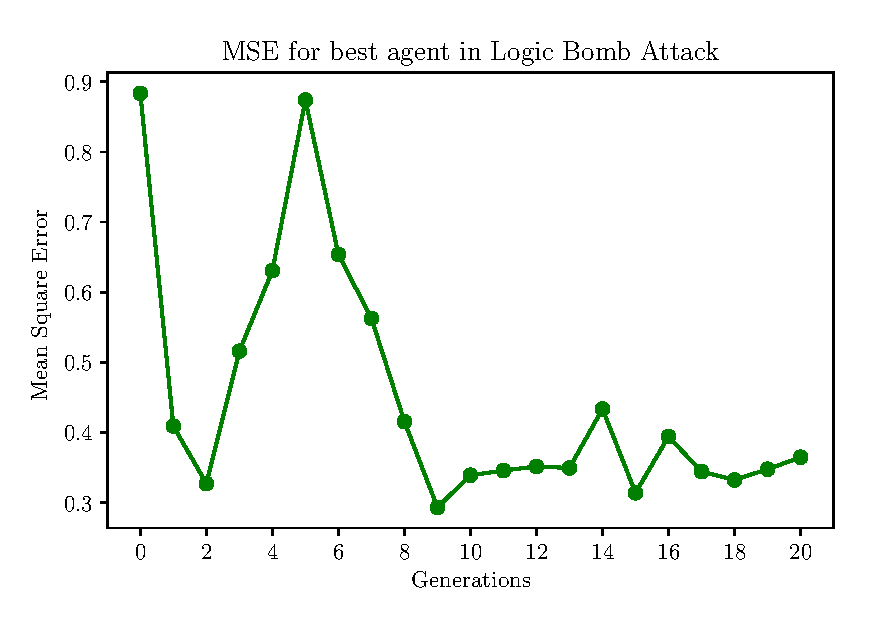
\includegraphics[scale=0.5]{figs/results/reward_best_agent_final.eps}
\vspace{-0.5cm}
\caption{MSE for the best agent in each generation using an algorithm to evolve neural networks}
\label{fig:reward_top_agent}
\end{figure}


On the other hand, an agent that kills all the processes will also reduce the effect of the threat, but the instance will be unusable which is not the goal of this study. Figure \ref{fig:processes_killed_top_agent} shows how the number of processes killed by the best agent are reduced in each generation, which means it is reducing the effect of the threat while killing the right process (malicious).\\

\begin{figure}[h!]
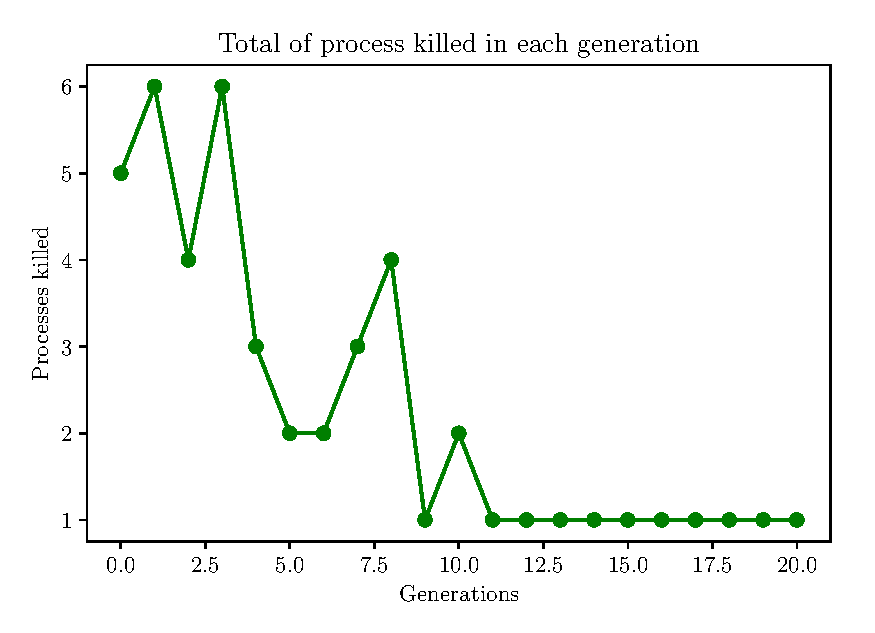
\includegraphics[scale=0.5]{figs/results/number_process_final_top_agent.eps}
\vspace{-0.5cm}
\caption{MSE for the best agent in each generation using an algorithm to evolve neural networks}
\label{fig:processes_killed_top_agent}
\end{figure}


\section{Conclusions}

In this paper, a new method for reducing the impact of cyber attacks, as well as the application of neuroevolution algorithms in cyber security, has been presented. The results of other researchers \cite{autoencoderdos, autoencoder1, autoencoder3} using autoencoders to classify cyber attacks have been confirmed, although a different methodology and type of cyber attack were used in this case. Autoencoders can provide a measure of how close a virtual instance is to a healthy state, allowing the combination of this measure with a neuroevolution algorithm to select the best agents, resulting in an innovative hybrid algorithm capable of detecting malicious processes running in a shell.
A hybrid method for detecting and mitigating malicious processes on simulated network systems in real-time is presented in this paper. By combining deep neural networks and evolutionary algorithms with an autoencoder-based fitness function, anomalous behavior in each device connected to the network is able to be detected. Using a virtual network and open source libraries, the behavior of malicious processes was studied and effective methods for detecting and responding to them were developed. Results show that the proposed approach is successful in detecting and terminating malicious processes, returning the virtual instances to their normal states as determined by an autoencoder-based fitness function. This work represents a promising direction for future research in the field of cybersecurity and deep neuroevolution.

\appendix
\section{Appendix: Description of each variable}\label{appx_variables}

\subsection{Central Processing Unit (CPU) Features}

\textbf{cpu\_cores:} The number of CPU cores present on the host. The non-normalized percentages will have a maximum value of 100\% $\cdot$ cores. The normalized percentages already take this value into account and have a maximum value of 100\%.\\

\textbf{cpu\_user\_pct:} The percentage of CPU time spent in user space. On multi-core systems, you can have percentages that are greater than 100\%. For example, if 3 cores are at 60\% use, then the system.cpu.user.pct will be 180\%.\\

\textbf{cpu\_system\_pct:} The percentage of CPU time spent in kernel space.\\

\textbf{cpu\_nice\_pct:} The percentage of CPU time spent on low-priority processes.\\

\textbf{cpu\_idle\_pct:} The percentage of CPU time spent idle.\\

\textbf{cpu\_iowait\_pct:} The percentage of CPU time spent in wait (on disk).\\

\textbf{cpu\_irq\_pct:} The percentage of CPU time spent servicing and handling hardware interrupts.\\

\textbf{cpu\_softirq\_pct:} The percentage of CPU time spent servicing and handling software interrupts.\\

\textbf{cpu\_steal\_pct:} The percentage of CPU time spent in involuntary wait by the virtual CPU while the hypervisor was servicing another processor.\\

\textbf{cpu\_total\_pct:} The percentage of CPU time spent in states other than Idle and IOWait.\\


\subsection{Core features}

\textbf{core\_user\_pct:} The percentage of CPU time spent in user space.\\

\textbf{core\_system\_pct:} The percentage of CPU time spent in kernel space.\\

\textbf{core\_nice\_pct:} The percentage of CPU time spent on low-priority processes.\\

\textbf{core\_idle\_pct:} The percentage of CPU time spent idle..\\

\textbf{core\_iowait\_pct:} The percentage of CPU time spent in wait (on disk).\\

\textbf{core\_irq\_pct:} The percentage of CPU time spent servicing and handling hardware interrupts.\\

\textbf{core\_softirq\_pct:}The percentage of CPU time spent servicing and handling software interrupts.\\

\textbf{core\_steal\_pct:}  The percentage of CPU time spent in involuntary wait by the virtual CPU while the hypervisor was servicing another processor. Available only on Unix.


\subsection{Disk Input/Output (Disk I/O) features}

\textbf{diskio\_read\_count:} The total number of reads completed successfully.\\

\textbf{diskio\_write\_count:} The total number of writes completed successfully.\\

\textbf{diskio\_read\_bytes:} The total number of bytes read successfully. On Linux this is the number of sectors read multiplied by an assumed sector size of 512.\\

\textbf{diskio\_write\_bytes:} The total number of bytes written successfully. On Linux this is the number of sectors written multiplied by an assumed sector size of 512.\\

\textbf{diskio\_read\_time:} The total number of milliseconds spent by all reads.\\

\textbf{diskio\_write\_time:} The total number of milliseconds spent by all writes.\\

\textbf{diskio\_io\_time:} The total number of of milliseconds spent doing I/Os.\\

\textbf{diskio\_iostat\_read\_request\_merges\_per\_sec:} The number of read requests merged per second that were queued to the device.\\

\textbf{diskio\_iostat\_write\_request\_merges\_per\_sec:} The number of write requests merged per second that were queued to the device.\\

\textbf{diskio\_iostat\_read\_request\_per\_sec:} The number of read requests that were issued to the device per second.\\

\textbf{diskio\_iostat\_wirte\_request\_per\_sec:} The number of write requests that were issued to the device per second.\\

\textbf{diskio\_iostat\_read\_per\_sec\_bytes:} The number of Bytes read from the device per second.\\

\textbf{diskio\_iostat\_read\_await:} The average time spent for read requests issued to the device to be served.\\

\textbf{diskio\_iostat\_write\_per\_sec\_bytes:}  The number of Bytes write from the device per second.\\

\textbf{diskio\_iostat\_write\_await:} The average time spent for write requests issued to the device to be served.\\

\textbf{diskio\_iostat\_request\_avg\_size:} The average size (in bytes) of the requests that were issued to the device.\\

\textbf{diskio\_iostat\_queue\_avg\_size:}The average queue length of the requests that were issued to the device.\\

\textbf{diskio\_iostat\_await:} The average time spent for requests issued to the device to be served.\\

\textbf{diskio\_iostat\_service\_time:} The average service time (in milliseconds) for I/O requests that were issued to the device.\\

\textbf{diskio\_iostat\_busy:} Percentage of CPU time during which I/O requests were issued to the device (bandwidth utilization for the device). Device saturation occurs when this value is close to 100\%.\\


\subsection{Entropy}

\textbf{entropy\_available\_bits:} The available bits of entropy.\\

\textbf{entropy\_pct:} The percentage of available entropy, relative to the pool size of 4096.\\



\subsection{Filesystem}

\textbf{filesystem\_available:} The disk space available to an unprivileged user in bytes.\\

\textbf{filesystem\_files:} The total number of file nodes in the file system.\\

\textbf{filesystem\_free:} The disk space available in bytes.\\

\textbf{filesystem\_free\_files:} The number of free file nodes in the file system.\\

\textbf{filesystem\_total:} The total disk space in bytes.\\

\textbf{filesytem\_used\_bytes:} The used disk space in bytes.\\

\textbf{filesystem\_used\_pct:} The percentage of used disk space.\\

\textbf{fsstat\_count:} Number of file systems found.\\

\textbf{fsstat\_total\_files:} Total number of files.\\

\textbf{fsstat\_total\_size\_free:} Total free space.\\

\textbf{fsstat\_total\_size\_used:} Total used space.\\

\textbf{fsstat\_total\_size\_total:} Total space (used plus free).\\

\subsection{Memory Swap}

\textbf{memory\_swap\_pct:} Total swap memory.\\

\textbf{memory\_swap\_used\_bytes:} Used swap memory in bytes.\\

\textbf{memory\_swap\_free:} Available swap memory.\\

\textbf{memory\_swap\_used\_pct:} The percentage of used swap memory.\\


\subsection{Memory hugepages}

\textbf{memory\_hugepages\_total:} Number of huge pages in the pool.\\

\textbf{memory\_hugepages\_used\_bytes:} Memory used in allocated huge pages in bytes.\\

\textbf{memory\_hugepages\_used\_pct:} Percentage of huge pages used.\\

\textbf{memory\_hugepages\_free:} Number of available huge pages in the pool.\\

\textbf{memory\_hugepages\_reserved:} Number of reserved but not allocated huge pages in the pool.\\

\textbf{memory\_hugepages\_surplus:} Number of overcommited huge pages.\\

\textbf{memory\_hugepages\_default\_size:} Default size for huge pages.




\subsection{Socket summary}

\textbf{socket\_summary\_all\_count:} All open connections.\\

\textbf{socket\_summary\_all\_listening:} All listening ports.\\

\textbf{socket\_summary\_tcp\_memory:} Memory used by  \textit{Transmission Control Protocol} (TCP) sockets in bytes, based on number of allocated pages and system page size.

\textbf{socket\_summary\_tcp\_all\_orphan:} A count of all orphaned tcp sockets.\\

\textbf{socket\_summary\_tcp\_all\_count:} All open TCP connections.\\

\textbf{socket\_summary\_tcp\_all\_listening:} All TCP listening ports.\\

\textbf{socket\_summary\_tcp\_all\_established:} Number of established TCP connections.\\

\textbf{socket\_summary\_tcp\_all\_close\_wait:} Number of TCP connections in \textit{close\_wait} state.\\

\textbf{socket\_summary\_tcp\_all\_time\_wait:} Number of TCP connections in \textit{time\_wait} state.\\

\textbf{socket\_summary\_udp\_memory:} Memory used by UDP sockets in bytes, based on number of allocated pages and system page size.\\

\textbf{socket\_summary\_udp\_all\_count:} All open UDP connections.\\


%================== Appendix II =====================% 

\section{Appendix: Description of each variable for the agents.}


\subsubsection{File descriptors}

\textbf{process\_fd\_limit\_hard:} limit hard on the number of file descriptors opened by the process. The hard limit can only be increased by root.\\

\textbf{process\_fd\_limit\_soft:} limit soft on the number of file descriptors opened by the process. The process can change the limit soft at any time.\\

\textbf{process\_fd\_open:} the number of file descriptors opened by the process.\\


\subsubsection{Central Processing Unit (CPU)}

\textbf{process\_cpu\_total\_norm\_pct:} Percentage of CPU time that the process consumes since the last event. This value is normalized by the number of CPU cores and ranges from 0\% to 100\%.\\

\subsubsection{Memory}

\textbf{process\_memory\_size:} The total in bytes of virtual memory that the process has.\\

\textbf{process\_memory\_rss\_bytes:} The Resident Set Size (RSS) in bytes. The proportion of memory used by a process that is held in main memory (RAM), that is, the memory that the process occupied in main memory or RAM.\\

\textbf{process\_memory\_share:} the shared memory in bytes that the process uses.\\

\subsubsection{Temporal features}

\textbf{process\_cpu\_start\_time\_seconds:} The time (in seconds) since the process started.



\bibliographystyle{plain} % We choose the "plain" reference style
\bibliography{references} % Entries are in the refs.bib file


%% Loading bibliography style file
%\bibliographystyle{model1-num-names}
%\bibliographystyle{iosart2c}

% Loading bibliography database
%\bibliography{iosart2c}



\end{document}
